\documentclass[aspectratio=169,t]{beamer}
\usefonttheme[onlymath]{serif}
\usepackage{xcolor}

%xcolor base colors:
%	black
%	blue
%	brown
%	cyan
%	lime
%	magenta
%	olive
%	orange
%	pink
%	purple
%	red
%	teal
%	violet
%	white
%	yellow

\definecolor{MyDarkGray}{gray}{0.33}

\definecolor{NavyBlue}{rgb}			{0,      0,    .502}
\definecolor{DarkMidnightBlue}{rgb}	{0,     .2,    .4}
\definecolor{DarkCerulean}{rgb}		{.0313, .2695, .4922}

\definecolor{MyTeal}{rgb}	{0, 	.5, 	.5}		%teal = 0,127,127
\definecolor{MyLtTeal}{rgb}	{.8125, .9375, 	.9375}	%lt.teal = 207,239,239
\definecolor{MySand}{rgb}	{1, 	.625, 	0}		%sand = 255,159,0
\definecolor{MyLtSand}{rgb}	{1, 	.9766, 	.875}	%lt.sand = 255,249,223
\definecolor{MyCoral}{rgb}	{1, 	.375, 	.375}	%coral = 255,96,96
\definecolor{MyLtCoral}{rgb}{1, 	.875, 	.875}	%lt.coral = 255,223,223

\usepackage[utf8]{inputenc}
\usepackage{graphicx}
\usepackage{subcaption}
\usepackage{color}
\usepackage{graphicx}
\usepackage{fancybox}
\usepackage[vlined]{algorithm2e}
\usepackage{anyfontsize}
\usepackage{standalone}
\usepackage{cancel}
\newcommand\hcancel[2][black]{\setbox0=\hbox{$#2$}\rlap{\raisebox{.45\ht0}{\textcolor{#1}{\rule{\wd0}{1pt}}}}#2}
\usepackage{tikz}
\usetikzlibrary{shapes,arrows.meta}
\tikzset{%
	>={Latex[width=2mm,length=2mm]},
	%Colors
	blackStyle/.style = {draw=black, fill=lightgray},
	tealStyle/.style = {draw=MyTeal, fill=MyLtTeal},
	coralStyle/.style = {draw=MyCoral, fill=MyLtCoral},
	sandStyle/.style = {draw=MySand, fill=MyLtSand},
	%Base Styles
	base/.style = {
		draw=black, fill=white, thick,
		text centered, font=\sffamily, inner sep=0mm},
	baseVox/.style = {base, circle,
		minimum width=1mm, minimum height=1mm},
	baseLine/.style = {thick},
}
\pgfdeclarelayer{bg}    % declare background layer
\pgfsetlayers{bg,main}  % set the order of the layers (main is the standard layer)
\newcommand{\rbar}{\hspace{1ex}\rvert\hspace{1ex}}

\usepackage{beamerthemesplit}
\usetheme[compress]{Heidelberg}
\definecolor{unirot}{rgb}{0.5976525,0,0}
\usecolortheme[named=unirot]{structure}

\title{Discrete Morse Theory}
\author{Bryan Wolfford}

\institute[Uni HD]{
	Universität Heidelberg\\
	Interdisciplinary Center for Scientific Computing\\
	Forensic Computational Geometry Laboratory\\
	\color{unirot}{wolfford@stud.uni-heidelberg.de}
}
\date{\today}

\begin{document}
\setlength{\intextsep}{0pt}
\def\hilite<#1>{\temporal<#1>{\color{black}}{\color{unirot}}{\color{gray}}}

%------------------------------------------------
\frame[plain]{
	\titlepage
}
\iffalse
%------------------------------------------------
\frame{\frametitle{Outline}
	\begin{itemize}
		\item Motivation \& Background
		\begin{itemize}
			\item Digital Images as Cubical Complexes
			\item Computational Topology
		\end{itemize} \pause
		\item Discrete Morse Theory
		\begin{itemize}
			\item Morse Theory and Simple Homotopy
			\item Discrete Morse Functions and Vector Fields 
			\item Gradient Fields as V-Paths
			%\item Morse Chain Complexes
		\end{itemize} \pause
		\item Examples \& Conclusions		
		\begin{itemize}
			\item Process Lower Star of a voxel
			\item 2D and 3D Persistent Homology Analysis
			\item Struture Simplification
		\end{itemize}
	\end{itemize}
}


%================================================
%================================================
\section{Motivation \& Background}

%------------------------------------------------
%TODO: populate 
\frame{\frametitle{Motivation}
	\begin{columns}[T]
		\begin{column}{.33\textwidth}
%			quantitative analysis of large 3D images. 
%			geometric: volume, surface area, curvature
%			Topological information is independent of geometric measures
%			however, computational topology require a combinatorial complex (huge)
%
%			A grayscale digital image, which are functions defined on a discrete lattice
%			cubical Complex, scale as O(n^3)
%			Morse complex same topological information, encodes topo.changes in level sets
%
%			Morse Theory
%				partions landscape into hills and dales
%				relates critical points to topology of manifold using negative gradient flow
%				Cells in Morse Complex defined by uniform flow behavior
%					Stable  manifolds:
%					droplets flow to same minimums (dales and basins)
%					boundries between basins are ridgeline passing thorugh saddles
%					maxima point where several basins touch
%					Unstable: 
%					regions where flow lines have same origin
%					intersection of two = Morse-Smale copmlex
%			
%			Continuous into discrete involves:
%				adapting to non-smooth unctions and manifolds
%				defining critical points
%				approx. gradient flow
%				devising efficient algs.
				
%			Discrete Morse Theory by Forman
%				gradient arrows one-to-one pairing of cells with faces
%				unpaired cells are critical points
%				<prese Cpm[lex arise from flow path between critical cells
		\end{column}
	\end{columns}
}

%------------------------------------------------
\frame{\frametitle{3D Grayscale Digital Images}
	\begin{columns}[T]
		\begin{column}{.66\textwidth}
			$g : D \rightarrow \mathbb{R}$ where $D \subset \mathbb{Z}^3$ is rectangular subset of the discrete lattice$^\dagger$:
			\[\hspace{2ex}D = \{(i,j,k) \rbar 0 \leq i \leq I,\hspace{1ex} 0 \leq j \leq J,\hspace{1ex} 0 \leq k \leq K\} \]
			A point $x \in D$ is called a {\color{MyTeal}voxel} (or pixel in 2D). \\
			\vspace{3.0\baselineskip}
			{\color{MyDarkGray}$^\dagger$The equations and algorithms apply with only minor adjustments to 2D digital images.}
		\end{column}
		\begin{column}{.33\textwidth}
			\centering
			\includegraphics[width=\textwidth]{figures/gimp/galeCrater_Mars.png}\\
			Gale Crater, Mars. \\
			{\scriptsize MOLA/HIRISE/NASA/JPL-Caltech/ASU/UA}
		\end{column}
	\end{columns}
}

%------------------------------------------------
\frame{\frametitle{p-cells and $K$}
	\begin{columns}[T]
		\begin{column}{.5\textwidth}
			$K$ is collection of all \emph{p-cells} built from voxels in D, with $p = \{0, 1, 2, 3\}$
			\begin{itemize}
				\only<1>{
					\item ({\color{MyTeal}0-cells}) are vertices (i.e. voxels)
				}\only<2>{
					\item (0-cells) are vertices (i.e. voxels)
					\item ({\color{MyTeal}1-cells}) are unit edges between voxels
				}\only<3>{ 
					\item (0-cells) are vertices (i.e. voxels)
					\item (1-cells) are unit edges between voxels
					\item ({\color{MyTeal}2-cells}) are unit squares
				}\only<4>{
					\item (0-cells) are vertices (i.e. voxels)
					\item (1-cells) are unit edges between voxels
					\item (2-cells) are unit squares
					\item ({\color{MyTeal}3-cells}) are unit cubes
				}
			\end{itemize}
		\end{column}
		\begin{column}{.5\textwidth}
			\centering
			\begin{tikzpicture}[node distance=0mm]
			\only<1>{
				\foreach \x in {-12mm,  8mm, 28mm}
					\foreach \y in {-16mm,  4mm, 24mm}
						\draw[tealStyle](\x,\y) circle[radius=1mm];

				\foreach \x in {-20mm,  0mm, 20mm}
					\foreach \y in {-20mm,  0mm, 20mm}
						\draw[tealStyle](\x,\y) circle[radius=1mm];

				\foreach \x in {-28mm, -8mm, 12mm}
					\foreach \y in {-24mm, -4mm, 16mm}
						\draw[tealStyle](\x,\y) circle[radius=1mm];
			}\only<2->{
				\foreach \x in {-12mm,  8mm, 28mm}
					\foreach \y in {-16mm,  4mm, 24mm}
						\draw[blackStyle](\x,\y) circle[radius=1mm];

				\foreach \x in {-20mm,  0mm, 20mm}
					\foreach \y in {-20mm,  0mm, 20mm}
						\draw[blackStyle](\x,\y) circle[radius=1mm];

				\foreach \x in {-28mm, -8mm, 12mm}
					\foreach \y in {-24mm, -4mm, 16mm}
						\draw[blackStyle](\x,\y) circle[radius=1mm];
			}\only<2>{
				\foreach \x in {-12mm,  8mm, 28mm}
					\draw[baseLine, tealStyle](\x,-16mm) -- (\x, 24mm);
				\foreach \x in {-20mm,  0mm, 20mm}
					\draw[baseLine, tealStyle](\x,-20mm) -- (\x, 20mm);
				\foreach \x in {-28mm, -8mm, 12mm}
					\draw[baseLine, tealStyle](\x,-24mm) -- (\x, 16mm);
				
				\foreach \y in {-16mm,  4mm, 24mm}
					\draw[baseLine, tealStyle](-12mm,\y) -- ( 28mm,\y);
				\foreach \y in {-20mm,  0mm, 20mm}
					\draw[baseLine, tealStyle](-20mm,\y) -- ( 20mm,\y);
				\foreach \y in {-24mm, -4mm, 16mm}
					\draw[baseLine, tealStyle](-28mm,\y) -- ( 12mm,\y);
				
				\draw[baseLine, tealStyle](-12mm,-16mm) -- (-28mm,-24mm);
				\draw[baseLine, tealStyle](  8mm,-16mm) -- ( -8mm,-24mm);
				\draw[baseLine, tealStyle]( 28mm,-16mm) -- ( 12mm,-24mm);
				
				\draw[baseLine, tealStyle](-12mm,  4mm) -- (-28mm, -4mm);
				\draw[baseLine, tealStyle](  8mm,  4mm) -- ( -8mm, -4mm);
				\draw[baseLine, tealStyle]( 28mm,  4mm) -- ( 12mm, -4mm);
				
				\draw[baseLine, tealStyle](-12mm, 24mm) -- (-28mm, 16mm);
				\draw[baseLine, tealStyle](  8mm, 24mm) -- ( -8mm, 16mm);
				\draw[baseLine, tealStyle]( 28mm, 24mm) -- ( 12mm, 16mm);
			}\only<3->{
				\foreach \x in {-12mm,  8mm, 28mm}
					\draw[baseLine, blackStyle](\x,-16mm) -- (\x, 24mm);
				\foreach \x in {-20mm,  0mm, 20mm}
					\draw[baseLine, blackStyle](\x,-20mm) -- (\x, 20mm);
				\foreach \x in {-28mm, -8mm, 12mm}
					\draw[baseLine, blackStyle](\x,-24mm) -- (\x, 16mm);
				
				\foreach \y in {-16mm,  4mm, 24mm}
					\draw[baseLine, blackStyle](-12mm,\y) -- ( 28mm,\y);
				\foreach \y in {-20mm,  0mm, 20mm}
					\draw[baseLine, blackStyle](-20mm,\y) -- ( 20mm,\y);
				\foreach \y in {-24mm, -4mm, 16mm}
					\draw[baseLine, blackStyle](-28mm,\y) -- ( 12mm,\y);
				
				\draw[baseLine, blackStyle](-12mm,-16mm) -- (-28mm,-24mm);
				\draw[baseLine, blackStyle](  8mm,-16mm) -- ( -8mm,-24mm);
				\draw[baseLine, blackStyle]( 28mm,-16mm) -- ( 12mm,-24mm);
				
				\draw[baseLine, blackStyle](-12mm,  4mm) -- (-28mm, -4mm);
				\draw[baseLine, blackStyle](  8mm,  4mm) -- ( -8mm, -4mm);
				\draw[baseLine, blackStyle]( 28mm,  4mm) -- ( 12mm, -4mm);
				
				\draw[baseLine, blackStyle](-12mm, 24mm) -- (-28mm, 16mm);
				\draw[baseLine, blackStyle](  8mm, 24mm) -- ( -8mm, 16mm);
				\draw[baseLine, blackStyle]( 28mm, 24mm) -- ( 12mm, 16mm);
			}\only<3>{
				\begin{pgfonlayer}{bg}
					\draw[draw=none,fill=MyLtTeal](-28mm,-24mm) -- (-28mm, 16mm) -- (-12mm, 24mm) -- ( 28mm, 24mm) -- ( 28mm,-16mm) -- ( 12mm,-24mm) -- cycle;
    			\end{pgfonlayer}
			}\only<4->{
				\begin{pgfonlayer}{bg}
					\draw[draw=none,fill=MyTeal](-28mm,-24mm) -- (-28mm, 16mm) -- (-12mm, 24mm) -- ( 28mm, 24mm) -- ( 28mm,-16mm) -- ( 12mm,-24mm) -- cycle;
    			\end{pgfonlayer}
			}
			\end{tikzpicture} \\
			\begin{flushleft}\footnotesize
				\only<1>{
					$K = \{$27 0-cells, $\ldots\}$
				}\only<2>{
					$K = \{$27 0-cells, 54 1-cells, $\ldots\}$
				}\only<3>{ 
					$K = \{$27 0-cells, 54 1-cells, 32 2-cells, $\ldots\}$
				}\only<4>{
					$K = \{$27 0-cells, 54 1-cells, 32 2-cells, 8 3-cells$\}$ \\
					$|K| = 121$
				}
			\end{flushleft}
		\end{column}
	\end{columns}
}

%------------------------------------------------
\frame{\frametitle{Faces, Cofaces, and Complexes}
	\begin{columns}[T]
		\begin{column}{.66\textwidth}
			\begin{itemize}
				\item $\alpha^{(p)}$ is a cell of p-th dimension
				\item A cell $\alpha^{(p)} \in K$ is a {\color{MyTeal}face} of another cell $\beta^{(q)}$ if:
				\begin{itemize}
					\item $p < q$, and 
					\item the vertices of $\alpha$ are a subset of the vertices of $\beta$
					\item written as $\alpha^{(p)} < \beta^{(q)}$. 
				\end{itemize}
				\item We can also say that $\beta$ is a {\color{MyTeal}coface} of $\alpha$.
				\item A set of cells $S \subset K$ is a {\color{MyTeal}complex}, if for any $\alpha \in S$, all its faces are also in $S$.
			\end{itemize}
		\end{column}
		\begin{column}{.33\textwidth}
		\end{column}
	\end{columns}
}

%------------------------------------------------
%TODO:circls for minimum not exactly right
\frame{\frametitle{Critical Points}
	\begin{columns}[T]
		\begin{column}{.25\textwidth}
			\centering
			\includegraphics[width=\textwidth]{figures/gimp/criticalPoints_minimum.png}\\
			Minimum $\bigcirc\hspace{-1.65ex}\circ$
		\end{column}
		\begin{column}{.25\textwidth}
			\centering
			\includegraphics[width=\textwidth]{figures/gimp/criticalPoints_saddle.png}\\
			Saddle $\oplus$
		\end{column}
		\begin{column}{.25\textwidth}
			\centering
			\includegraphics[width=\textwidth]{figures/gimp/criticalPoints_maximum.png}\\
			Maximum $\odot$
		\end{column}
		\begin{column}{.25\textwidth}
			\centering
			\includegraphics[width=\textwidth]{figures/gimp/criticalPoints_monkeySaddle.png}\\
			Monkey Saddle $\otimes$
		\end{column}
	\end{columns}
}

%------------------------------------------------
\frame{\frametitle{Gaussian Landscape}
	\begin{columns}[T]
		\begin{column}{.5\textwidth}
			\centering
			\includegraphics[width=\textwidth]{figures/gimp/gaussianLandscape.png} \\
			3 minima (lakes) \\
			15 saddles (passes) \\
			13 maxima (peaks)
		\end{column}
		\begin{column}{.5\textwidth}
			\includegraphics[width=\textwidth]{figures/gimp/criticalPoints.png}
		\end{column}
	\end{columns}
}

%------------------------------------------------
\frame{\frametitle{Lower Level Cuts}
	\begin{columns}[T]
		\begin{column}{.66\textwidth}
			A {\color{MyTeal}lower level cut} is the set of all voxels with grayscale values less than some threshold $t$:
			\[ D_t = \{x \in D \rbar g(x) \leq t\}\]
			or for a cubical complex:
			\[ K_t = \{\alpha \in K \rbar g(x) \leq t, \forall x \in \alpha\}\]
		\end{column}
	\end{columns}
}


%------------------------------------------------
%TODO: add in persistant homology once slide is made
\frame{\frametitle{Filtration}
	\begin{itemize}
		\item The topology of the lower level cuts changes as the threshold is varied.
		\begin{itemize}
			\item $t < \min{g(x) \rbar x \in K}$, $K_t = \{\varnothing\}$; 
			\item as $t$ increases, cells are added so that \\
				  for any $t_1 < t_2$, $K_{t_1}$ is a subcomplex of $K_{t_2}$
			\item $t > \max{g(x) \rbar x \in K}$, $K_t = K$.
		\end{itemize}
		\item Such a sequence of nested complexes is called a {\color{MyTeal}filtration}.
		%\item The changes in topology are quantified by computing the {\color{MyTeal}persistent homology} of the filtration.
	\end{itemize}
}

%------------------------------------------------
%TODO:images don't line up correctly
\frame{\frametitle{Lower Level Cuts of a Gaussian Landscape}
	\only<1>{
		$t \geq \max{g(\alpha)}$ \\
		\centering
		\includegraphics[width=.8\textwidth]{figures/gimp/gaussianLandscape.png}
	}\only<2>{
		$t \sim small$ \\
		\centering
		\includegraphics[width=.8\textwidth]{figures/gimp/excursionSet_a.png}
	}\only<3>{
		$t \sim medium$ \\
		\centering
		\includegraphics[width=.8\textwidth]{figures/gimp/excursionSet_b.png}
	}\only<4>{
		$t \sim large$ \\
		\centering
		\includegraphics[width=.8\textwidth]{figures/gimp/excursionSet_c.png}
	}\only<5>{
		$t \geq \max{g(\alpha)}$ \\
		\centering
		\includegraphics[width=.8\textwidth]{figures/gimp/gaussianLandscape.png}
	}
}

%------------------------------------------------
%TODO: populate
%\frame{\frametitle{Persistant Homology}
%}

%------------------------------------------------
\frame{\frametitle{Simple Homotopy}
	\begin{itemize}
		%\item Definitions are given for cubical complexes, but can be extended to general CW complexes.
		\item $\alpha$ is called the {\color{MyTeal}free face} of $\beta$, if $\alpha^{(p-1)}$ is a face of $\beta^{(p)}$, and $\alpha$ has no other cofaces. We then call $(\alpha, \beta)$ a {\color{MyTeal}free pair}. \pause
		\item An {\color{MyTeal}elementary collapse} of $K$ occurs when we remove a free pair from $K$, obtaining a subcomplex of $K$. \pause
		\item We say that $K$ {\color{MyTeal}collapses} to a $K'$ if there is a finite sequence of elementary collapses from $K$ to $K'$. \pause
		%\item If a cubical complex collapses to a point it is {\color{MyTeal}collapsible}.
		\item An {\color{MyTeal}expansion} is the inverse of a collapse.  \pause
		\item Two cubical complexes are {\color{MyTeal}simple homotopy equivalent} if there is a sequence of collapses and expansions from one complex to the other. \pause
		\item As elementary collapses determine strong deformation retractions if two cubical complexes are simple homotopy equivalent, then they are homotopy equivalent. 
	\end{itemize}
}

\fi
%------------------------------------------------
\frame{\frametitle{Discrete Morse Functions}
	A function, $f : K \rightarrow \mathbb{R}$ is a {\color{MyTeal}discrete Morse function} if %for every $\alpha^{(p)} \in K$, 
	%\begin{itemize}
	%	\item $f$ takes a value less than or equal to $f(\alpha)$ on at most one coface of $\alpha$, and 
	%	\item $f$ takes a value greater than or equal to $f(\alpha)$ on at most one face of $\alpha$. In other words,
	%\end{itemize}
	\vspace{-1\baselineskip}
	\begin{center}
		\[1 \geq \#\{\beta^{(p+1)} > \alpha \rbar f(\beta) \leq f(\alpha)\},\]
		and 
		\[1 \geq \# \{\gamma^{(p-1)} < \alpha \rbar f(\gamma) \geq  f(\alpha)\}.\]
	\end{center}
	A cell, $\alpha^{(p)}$ is {\color{MyTeal}critical} if all cofaces take strictly greater function values, and all faces take values which are strictly lower.
}

\iffalse
%------------------------------------------------
\frame{\frametitle{Non-Critical Cells}
	%\begin{columns}[T]
	%	\begin{column}{.66\textwidth}
			\begin{itemize}
				\item A cell $\alpha$ can only fail to be critical in two possible ways, either there can exist
				\begin{itemize}
					\item a $\gamma < \alpha$ such that $f(\gamma) \geq f(\alpha)$, or
					\item a $\beta > \alpha$ such that $f(\beta) \leq f(\alpha)$. 
				\end{itemize}
				\item these two possibilities cannot be true simultaneously for a given cell $\alpha$. 
				\item Thus each non-critical cell $\alpha$ may be paired either with 
				\begin{itemize}
					\item a non-critical cell that is a coface of $\alpha$, or
					\item a non-critical cell that is a face of $\alpha$.
				\end{itemize}
				\item It is not easy to construct discrete Morse functions on a given complex!
				%\item it is usually simpler to work with a discrete vector field.
			\end{itemize}
	%	\end{column}
	%	\begin{column}{.33\textwidth}
	%	\end{column}
	%\end{columns}
}

%------------------------------------------------
\frame{\frametitle{Discrete vector fields}
	%\begin{columns}[T]
	%	\begin{column}{.66\textwidth}
			\begin{itemize}
				\item A {\color{MyTeal}discrete vector field} $V$ is a collection of pairs $\{\alpha^{(p)} < \beta^{(p+1)}\}$ of cells in $K$ such that each cell is in at most one pair of $V$. 
				\item A discrete Morse function defines a discrete vector field by pairing $\alpha^{(p)} < \beta^{(p+1)}$ whenever $f(\beta) \leq f(\alpha)$. 
				\item The critical cells are precisely those that do not appear in any pair. 
				\item Discrete vector fields that arise from Morse functions are called {\color{MyTeal}gradient vector fields}.
			\end{itemize}
	%	\end{column}
	%	\begin{column}{.33\textwidth}
	%	\end{column}
	%\end{columns}
}

%------------------------------------------------
\frame{\frametitle{V-Path}
	%\begin{columns}[T]
	%	\begin{column}{.66\textwidth}
			\begin{itemize}
				\item A {\color{MyTeal}V-path} is the the flow-line of a vector field in the discrete setting.
				\item It is a sequence of cells: $\alpha^{(p)}_0, \beta^{(p+1)}_0, \alpha^{(p)}_1, \beta^{(p+1)}_1, \alpha^{(p)}_2, \ldots, \beta^{(p+1)}_{r-1}, \alpha^{(p)}_r $.
				\item where $(\alpha_i, \beta_i) \in V, \beta_i > \alpha_{i+1}$, and $\alpha_i \neq \alpha_{i+1}$ for all $i = 0, \ldots, r-1$. 
				\item A V-path is a {\color{MyTeal}non-trival closed V-path} if $\alpha_r = \alpha_0$ for $r \geq 1$. 
				\item A discrete vector field is the gradient vector field of a discrete Morse function \emph{if and only if} there are \textbf{no} non-trivial closed V-paths.
			\end{itemize}
	%	\end{column}
	%	\begin{column}{.33\textwidth}
	%	\end{column}
	%\end{columns}
}

%------------------------------------------------
\frame{\frametitle{The discrete Morse theory, simple homotopy connection}
	%\begin{columns}[T]
	%	\begin{column}{.66\textwidth}
			\begin{itemize}
				\item arises from the pairs in the gradient vector field. 
				\item the {\color{MyTeal}level subcomplex} $K(c)$ includes all cells with $f(\alpha) \leq c$ and all their faces:
				\item $K(c) = \cup_{f(\alpha) \leq c} \cup_{\gamma \leq \alpha} \gamma$
				\item a sequence of subcomplexes $K(c_i)$, for increasing values of $c_i$, defines a filtration which relates to simple homotopy theory.
			\end{itemize}
	%	\end{column}
	%	\begin{column}{.33\textwidth}
	%	\end{column}
	%\end{columns}
}


%TODO: define Morse chain complexes
%Lemma 1: If there are no critical simplices \alpha with f (\alpha) 2 (a, b], then K(b) collapses to K(a). The sequence of elementary collapses are defined by pairs (\alpha(p), (p+1) ) from the gradient vector field. Alternatively, if level subcomplexes (p) K(a) and K(b) differ by a single critical p-cell, , then we can define an attaching map on the boundary of (see Theorem 3.4 of [14]). Thus, a discrete Morse function on a cubical complex induces a CW-complex (Corollary 3.5 of [14]). Lemma 2: Let K be a cubical complex with discrete Morse function f . Then K is homotopy equivalent to a CW-complex X with exactly one cell of dimension p for each critical cell in K of dimension p. K We now define a discrete analogue of what is sometimes known as the “Thom-Smale-Witten” complex [29]. The result is an abstract chain complex that Forman calls the Morse complex, and that we call the Morse chain complex. Let Cp (K, Z2 ) be the group of p-chains with Z2 coefficients (see Sec. 2.2). Let Mp ✓ Cp (K, Z2 ) be the subgroup generated by the critical p-cells. We define a boundary map @p : Mp ! Mp 1 as follows. For any critical p-cell set @ = \alpha2Mp X 1 c\alpha, \alpha.  (5) The coefficients c\alpha, encapsulate the induced orientations and number of V -paths between the maximal (i.e. co-dimension-1) faces of and the critical (p 1)-cell \alpha, and are defined as follows. Let ( , \alpha) be the set of all V -paths from maximal faces of to \alpha. Because we compute homology with Z2 coefficients, orientations are ignored and c\alpha, =  ( 1 0 if if # # ( ( , , \alpha) \alpha) is is even.  odd,  (6) With the boundary operator so defined, we have the following result (see Section 8 of [14], or Section 7 of [15]). Theorem 3: Let Mp be the chain group of critical p- cells. The Morse chain complex 0 ! Mn !  @ n  Mn  1  @n  !1  . . . ! @ 0 M0 ! 0  (7) calculates the homology of K. That is, if we define Ker @p Hp(M, @) = Im @p+1 then for each p, Hp (M, @) ⇠  = Hp (K, Z2). This theorem implies that the persistent homology of the digital image can be computed from the Morse chain complex.



%------------------------------------------------
%------------------------------------------------
\section{The Algorithms}
%------------------------------------------------
\frame{\frametitle{The Algorithms}
	%\begin{columns}[T]
	%	\begin{column}{.66\textwidth}
			\begin{itemize}
				\item Our approach to characterizing the topology of the level cuts of a grayscale function proceeds in two stages. 
				\item First we construct a discrete vector field on the cubical cell complex using simple-homotopy expansions; 
				\item we use this vector field to build the Morse chain complex by following V-paths.
			\end{itemize}
	%	\end{column}
	%	\begin{column}{.33\textwidth}
	%	\end{column}
	%\end{columns}
}

%------------------------------------------------
\frame{\frametitle{Constructing the Discrete Vector Field}
	%\begin{columns}[T]
	%	\begin{column}{.66\textwidth}
			\begin{itemize}
				\item Recall a filtration of $K$ is the sequence of subcomplexes which contain the cells in K that have no vertex with a grayscale value greater than some threshhold $t$, corresponding to the lower level cuts of the digital image.
				\item The goal then is to construct a discrete Morse function on the cubical complex whose critical cells exactly match the changes in topology between successive elements of this filtration. 
				\item We achieve this by using simple homotopy expansions to grow from one subcomplex to the next, and introduce critical cells only when a simple homotopy pairing cannot be found.
			\end{itemize}
	%	\end{column}
	%	\begin{column}{.33\textwidth}
	%	\end{column}
	%\end{columns}
}

%------------------------------------------------
\frame{\frametitle{Lower-Star}
	%\begin{columns}[T]
	%	\begin{column}{.66\textwidth}
			\begin{itemize}
				\item When the $g$-values are unique %details in paper
				\item we know that the subcomplex $K_{t_i}$ differs from its predecessor in the filtration $K_{t_{i-1}}$ by the single voxel $x_i = g^{-1}(t_i)$ and the 1-, 2- and 3-cells for which $x_i$ is the highest valued voxel.
				\item This set of cells in the neighbourhood of $x_i$ is called the {\color{MyTeal}lower star}.
				\item \[ L(x) = \{\alpha \in K \rbar x \in \alpha \text{ and } g(x) = \max_{y \in \alpha}{g(y)}\}\]
				\item The lower stars of all voxels $x \in D$ form a disjoint partition of $K$.
			\end{itemize}
	%	\end{column}
	%	\begin{column}{.33\textwidth}
	%	\end{column}
	%\end{columns}
}

%------------------------------------------------
\frame{\frametitle{ProcessLowerStars}
	%\begin{columns}[T]
	%	\begin{column}{.66\textwidth}
			\begin{itemize}
				\item finds a sequence for adding the cells from $L(x_i)$ to $K_{t_{i-1}}$ to grow it into $K_{t_i}$%, for each voxel $x_i$. 
				%\item To avoid spurious critical cells, our algorithm aims to leave a minimal number of cells unpaired. This is achieved by utilising simple homotopic expansions where possible. 
				\item Since pairing occurs only between cells in the same lower star, each lower star can be treated independently, in parallel if need be. 
				%\item C and V (the lists of critical cells and discrete vector field pairs). 
				%\item When there is a single available unpaired face for the cell $\alpha$, we call this face {\color{MyTeal}$pair(\alpha)$}. 
				\item ProcessLowerStars is based on two priority queues of cells, PQone and PQzero, which require an ordering, $G(\alpha)$, of the cells in each lower star. 
				\item Any ordering based primarily on the maximal g value of the vertices of the cell and in which a cell is ranked after its faces will suffice, i.e. lexicographic ordering:
				\item Given $\alpha \in L(x)$, with vertices ${x, y_1, \ldots, y_k}$, define
					\[ G(\alpha) = (g(x), g(y_{i_1}), \dots, g(y_{i_k})) \text{ where } g(x) > g(y_{i_1}) > \ldots > g(y_{i_k}) \] 
			\end{itemize}
	%	\end{column}
	%	\begin{column}{.33\textwidth}
	%	\end{column}
	%\end{columns}
}

%------------------------------------------------
\frame{\frametitle{Process Lower Stars - Main Loop (1 of 6)}
	\begin{columns}[T]
		\begin{column}{.6\textwidth}
			$L(8) = \{8, 81, 82, 83, 8432, 86, 8653, 8762\}$ \\
			$C = \{\varnothing\}$ \\
			$V = \{\varnothing\}$ \\
			$PQone \hspace{.9ex}= \{\varnothing\}$ \\
			$PQzero = \{\varnothing\}$ \\
			\vspace{\baselineskip}
			{\color{MyDarkGray}The {\color{MyTeal}lower link} of vertex 8 is shown as {\color{black}dark edges}; these are the faces of cells in $L(8)$ that belong to the complex $K_7$}. 
		\end{column}
		\begin{column}{.4\textwidth}
			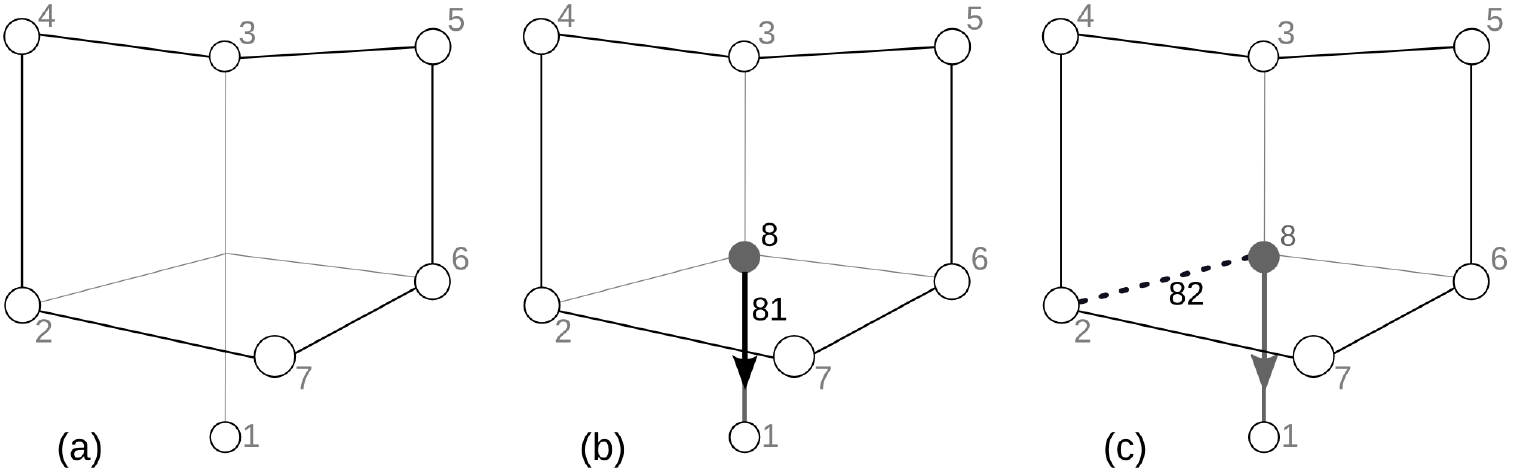
\includegraphics[width=\textwidth]{figures/gimp/processLowerStars_voxel_a.png}
		\end{column}
	\end{columns}
}

%------------------------------------------------
\frame{\frametitle{Process Lower Stars - Main Loop (2 of 6)}
	\begin{columns}[T]
		\begin{column}{.6\textwidth}
			$L(8) = \{\hcancel[MyCoral]{8, 81}, 82, 83, 8432, 86, 8653, 8762\}$ \\
			$C = \{\varnothing\}$ \\
			$V = \{{\color{MyTeal}81, 8}\}$ \\
			$PQone \hspace{.9ex}= \{\varnothing\}$ \\
			$PQzero = \{\varnothing\}$ \\
			\vspace{\baselineskip}
			{\color{MyDarkGray}First considered is the 0-cell $x$ itself. If $L(x)$ is empty, $x$ is a local minimum, therefore critical and added to $C$. Otherwise, $x$ is paired with its lowest incident edge.}\\
			\begin{enumerate}
				\item Here 8 is paired with 81.
			\end{enumerate}
		\end{column}
		\begin{column}{.4\textwidth}
			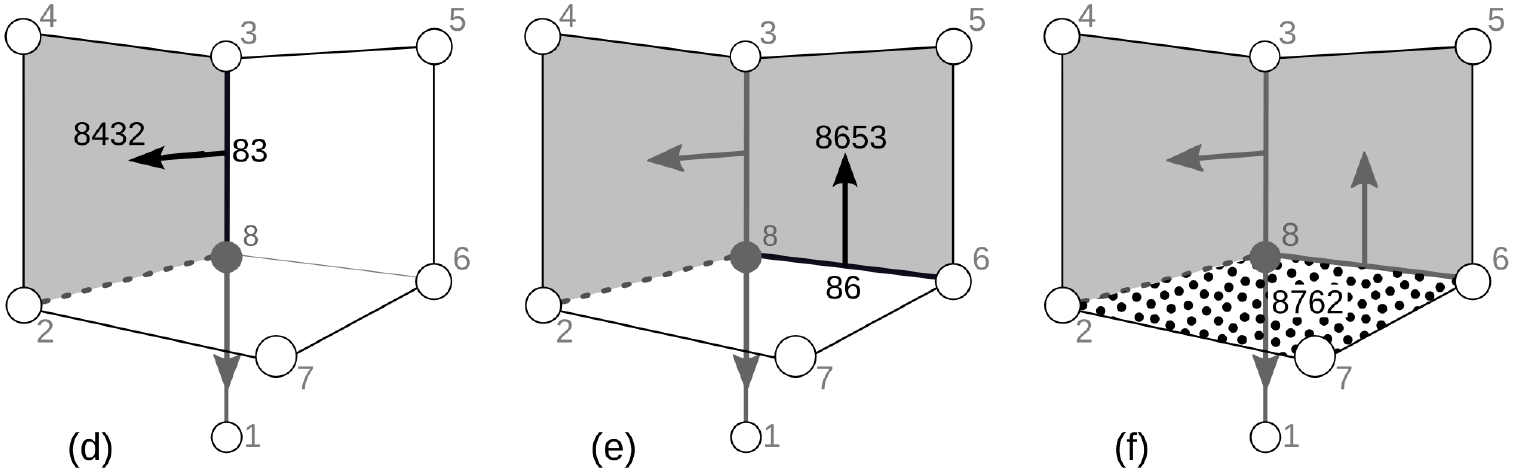
\includegraphics[width=\textwidth]{figures/gimp/processLowerStars_voxel_b.png}
		\end{column}
	\end{columns}
}

%------------------------------------------------
\frame{\frametitle{Process Lower Stars - Main Loop (3 of 6)}
	\begin{columns}[T]
		\begin{column}{.6\textwidth}
			$L(8) = \{\hcancel[MyCoral]{8, 81, 82, 83}, 8432, \hcancel[MyCoral]{86}, 8653, 8762\}$ \\
			$C = \{{\color{MyTeal}82}\}$ \\
			$V = \{81, 8\}$ \\
			$PQone \hspace{.9ex}= \{\varnothing\}$ \\
			$PQzero = \{{\color{MyTeal}\hcancel[MySand]{82}, 83, 86}\}$ \\
			\vspace{\baselineskip}
			{\color{MyDarkGray}Cell pairs are made from simple homotopy expansions. When expansions are no longer possible, a critical cell is created}
			\begin{enumerate}
				\setcounter{enumi}{1}
				\item Edges 82, 83, 86 are added to $PQzero$. %There are no cells adjacent to 81 with a single unpaired face so $PQone$ remains empty.
				\item 82 is popped from $PQzero$ and added to $C$; it is critical and marked as a dashed line.
			\end{enumerate}
		\end{column}
		\begin{column}{.4\textwidth}
			\includegraphics[width=\textwidth]{figures/gimp/processLowerStars_voxel_c.png}
		\end{column}
	\end{columns}
}

%------------------------------------------------
\frame{\frametitle{Process Lower Stars - Main Loop (4 of 6)}
	\begin{columns}[T]
		\begin{column}{.6\textwidth}
			$L(8) = \{\hcancel[MyCoral]{8, 81, 82, 83, 8432, 86}, 8653, \hcancel[MyCoral]{8762}\}$ \\
			$C = \{82\}$ \\
			$V = \{81, 8, {\color{MyTeal}8432, 83}\}$ \\
			$PQone \hspace{.9ex}= \{{\color{MyTeal}\hcancel[MySand]{8432}, 8762}\}$ \\
			$PQzero = \{\hcancel[MySand]{83}, 86\}$ \\
			\vspace{\baselineskip}
			{\color{MyDarkGray}Expansions continue from new critical cells.}
			\begin{enumerate}
				\setcounter{enumi}{3}
				\item Edge 82 has two cofaces 8432 and 8762 that are added to $PQone$.
				\item Square 8432 is popped from $PQone$, it is paired with its free face, edge 83.
			\end{enumerate}
		\end{column}
		\begin{column}{.4\textwidth}
			\includegraphics[width=\textwidth]{figures/gimp/processLowerStars_voxel_d.png}
		\end{column}
	\end{columns}
}

%------------------------------------------------
\frame{\frametitle{Process Lower Stars - Main Loop (5 of 6)}
	\begin{columns}[T]
		\begin{column}{.6\textwidth}
			$L(8) = \{\hcancel[MyCoral]{8, 81, 82, 83, 8432, 86, 8653, 8762}\}$ \\
			$C = \{82\}$ \\
			$V = \{81, 8, 8432, 83, {\color{MyTeal}8653, 86}\}$ \\
			$PQone \hspace{.9ex}= \{\hcancel[MySand]{{\color{MyTeal}8653}}, 8762\}$ \\
			$PQzero = \{\hcancel[MySand]{86}\}$ \\
			\vspace{\baselineskip}
			{\color{MyDarkGray}When a cell reaches the front of $PQone$ it is paired with its single available face.}
			\begin{enumerate}
				\setcounter{enumi}{5}
				\item Square 8653 is a coface of edge 83 and added to $PQone$.
				\item Square 8653 is then popped from $PQone$, and paired with edge 86.
			\end{enumerate}
		\end{column}
		\begin{column}{.4\textwidth}
			\includegraphics[width=\textwidth]{figures/gimp/processLowerStars_voxel_e.png}
		\end{column}
	\end{columns}
}

%------------------------------------------------
\frame{\frametitle{Process Lower Stars - Main Loop (6 of 6)}
	\begin{columns}[T]
		\begin{column}{.6\textwidth}
			$L(8) = \{\hcancel[MyCoral]{8, 81, 82, 83, 8432, 86, 8653, 8762}\}$ \\
			$C = \{82, {\color{MyTeal}8762}\}$ \\
			$V = \{81, 8, 8432, 83, 8653, 86\}$ \\
			$PQone \hspace{.9ex}= \{\hcancel[MySand]{8762}\}$ \\
			$PQzero = \{\hcancel[MySand]{{\color{MyTeal}8762}}\}$ \\
			\vspace{\baselineskip}
			\begin{enumerate}
				\setcounter{enumi}{7}
				\item Square 8762 is popped from $PQone$ and added to $PQzero$; as all its faces have been paired. 
				\item Square 8762 is popped from $PQzero$ and added to $C$. It is the critical 2-cell marked with spots.
			\end{enumerate}
		\end{column}
		\begin{column}{.4\textwidth}
			\includegraphics[width=\textwidth]{figures/gimp/processLowerStars_voxel_f.png}
		\end{column}
	\end{columns}
}



%------------------------------------------------
\frame{\frametitle{Sandstone ABCD}
	\begin{columns}[T]
		\begin{column}{\textwidth}
			\includegraphics[width=\textwidth]{figures/gimp/sandstone_abcd.png}
		\end{column}
	\end{columns}
}

%------------------------------------------------
\frame{\frametitle{Sandstone - Critical Cells}
	\begin{columns}[T]
		\begin{column}{.5\textwidth}
			\centering
			\includegraphics[width=.8\textwidth]{figures/gimp/sandstone_a.png}
		\end{column}
		\begin{column}{.5\textwidth}
			\centering
			\includegraphics[width=.8\textwidth]{figures/gimp/sandstone_b.png}
		\end{column}
	\end{columns}
}

%------------------------------------------------
\frame{\frametitle{Sandstone - Subsets}
	\begin{columns}[T]
		\begin{column}{.5\textwidth}
			\centering
			\includegraphics[width=.8\textwidth]{figures/gimp/sandstone_a.png}
		\end{column}
		\begin{column}{.25\textwidth}
			\includegraphics[width=\textwidth]{figures/gimp/sandstone_c.png}
		\end{column}
		\begin{column}{.2\textwidth}
			\includegraphics[width=\textwidth]{figures/gimp/sandstone_d.png}
		\end{column}
	\end{columns}
}

%------------------------------------------------
\frame{\frametitle{3D Foam}
	\begin{columns}[T]
		\begin{column}{.425\textwidth}
			\centering
			\includegraphics[width=\textwidth]{figures/gimp/foam.png}
		\end{column}
		\begin{column}{.575\textwidth}
			\begin{itemize}
				\item \hspace{1.75ex}262,144 voxels (64x64x64)
				\item 1,540,351 cells in the cubical complex
				\item \hspace{4ex}4,093 cells in the Morse complex
			\end{itemize}
		\end{column}
	\end{columns}
}

%------------------------------------------------
\frame{\frametitle{Outlook}
	\begin{columns}[T]
		\begin{column}{.5\textwidth}
			Data Compression
			Geographic Information Systems
			Medical Image Analysis
				Machine Learning
				Principle Componant Analysis
		\end{column}
	\end{columns}
}
\fi
\end{document}
